\chapter{RESULT}

\noindent\hspace{2.5em}We have used pre-recorded footage from CCTV cameras to analyze and compare the performance and accuracy of the detection and counting system. 

\vspace{1em}

\noindent\hspace{2.5em}To evaluate the accuracy of the model, we compared detection counts with manual counting over a ten-minute span of one video with every model we have. The aim of this is to see the accuracy and improvement of our model. The results in Table 4.1 shows the accuracy results of different models. Person and motorbike used YOLO pretrain model to detect these two classes, so the accuracy and considered constant throughout different models. Helmet detection rises from 42\% to 96\%, which is 54\% improvement from the first model to latest model. The calculation method of finding helemt detection accuracy across different models is to find the total ground truth and detection of the train model, then divide it to find the accuracy. We find the best confident for each model by comparing confident of 0.15 and 0.3 to find the best accuracy. Best17 model have the ground truth helmet of 60, we have the confident set to 0.15 and detected the detection number to be 55, which is 90\%. On the other hand, we change the confident to 0.3 and the results of the detection is 58, which is 95\% resulting in a better accuracy.

\vspace{1em}

\noindent\hspace{2.5em}After evaluating the model's detection accuracy, we proceeded to assess the performance of the counting system. This analysis was conducted using two pre-recorded CCTV footage videos. Tables 1.2 and 1.3 present the counting accuracy for helmeted and non-helmeted (head) riders, derived from Video 1 and Video 2 respectively. These tables utilize a double-line counting method.

\vspace{1em}
For the helmet and head detection specifically, we experimented with adjusting the length of the double-counting lines to evaluate their impact on counting accuracy. For instance, we tested line lengths such as 300 pixels for Line X and 450 pixels for Line Y, along with several other variations. The results indicated that optimal performance occurs when the length of the double lines is kept within approximately 150 pixels. Longer lines tended to increase the likelihood of multiple or false counts due to prolonged object overlap with the counting zone.

\vspace{1em}
In contrast, Tables 1.4 and 1.5 focus on motorbike and person counting accuracy, also based on Video 1 and Video 2. However, these use the BotSort tracking and counting method instead of the double-line approach. This separation allows us to compare the performance of different counting techniques across different object categories and scenarios.

\vspace{1em}
To evaluate counting accuracy, we use a relative error formula to calculate the percentage difference between the counted value and the ground truth. This approach provides a clear measure of overcounting or undercounting, allowing us to identify and analyze overflow or missed counts in the system.


\section{Model Result}
\noindent\textbf{Table 4.1} \\
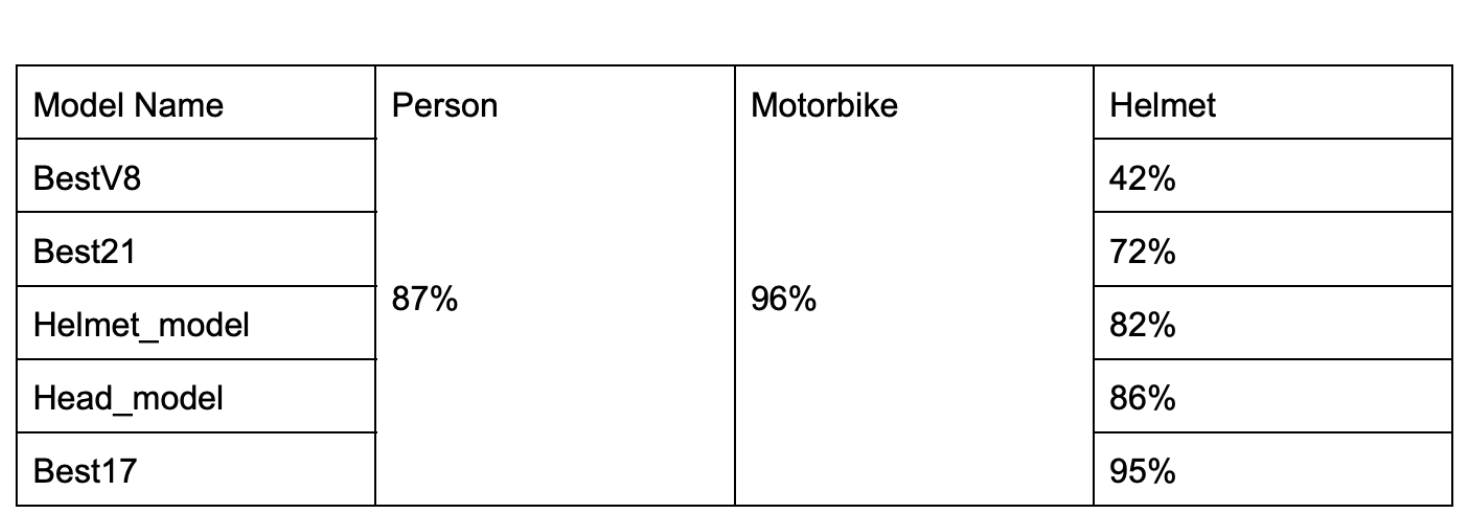
\includegraphics[width=1\textwidth]{model_result.png}
The figure presents the detection accuracy of various models across three object categories: person, motorbike, and helmet. The accuracy values for person and motorbike detection remain constant across models—87\% and 96\% respectively—because these classes were detected using the pretrained YOLO model without additional fine-tuning. In contrast, the helmet detection results vary significantly between models, as each represents a different version of a custom-trained helmet detection model.
\section{Counting Result}
\vspace{0.5em}
\noindent\textbf{Table 4.2} \\
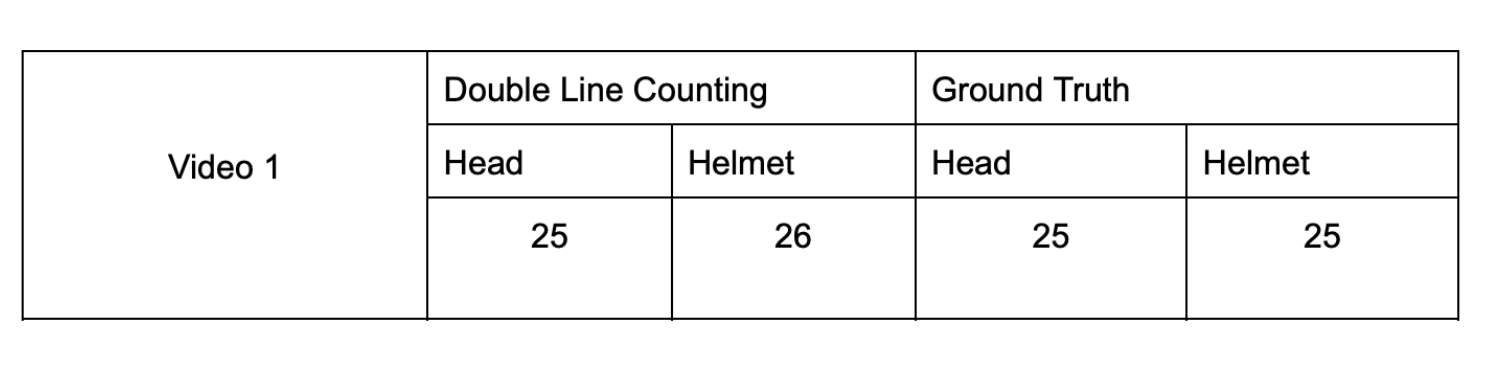
\includegraphics[width=1\textwidth]{test1.png}
Table 4.2 shows the counting results for Video 1 using the double-line method compared to the ground truth. The system accurately counted heads (25 vs. 25) but slightly overcounted helmets (26 vs. 25), likely due to duplicate detections or crossing artifacts.


\vspace{0.5em}
\noindent\textbf{Table 4.3} \\
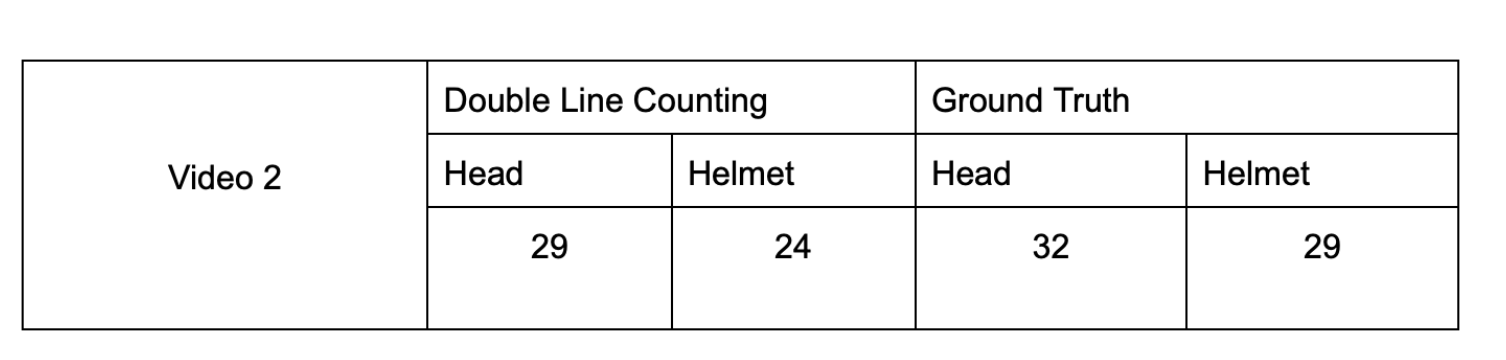
\includegraphics[width=1\textwidth]{test2.png}
Table 4.3 shows the double-line counting results for Video 2. The system counted 29 heads and 24 helmets, while the ground truth recorded 32 heads and 29 helmets. This indicates undercounting in both categories, which could be due to missed detections or rapid movements causing objects to skip the counting lines.


\vspace{0.5em}
\noindent\textbf{Table 4.4} \\
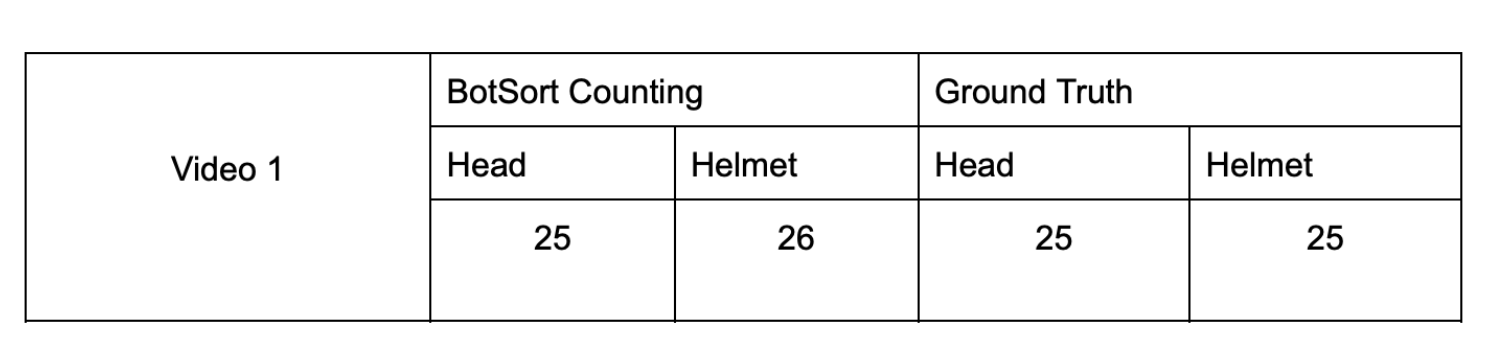
\includegraphics[width=1\textwidth]{test3.png}
Table 4.4 presents BotSort counting results for Video 1. The system detected 52 persons and 32 motorbikes, compared to the ground truth values of 51 persons and 30 motorbikes. This reflects a small overcount in both categories, likely due to brief tracking ID switches or overlapping detections in crowded scenes.

\newpage
\vspace{0.5em}
\noindent\textbf{Table 4.5} \\
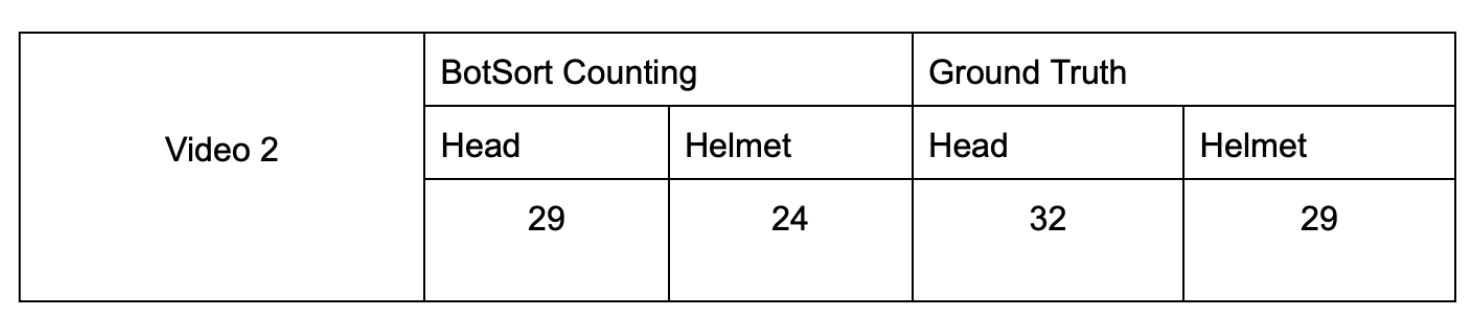
\includegraphics[width=1\textwidth]{test4.png}
Table 4.5 summarizes the BotSort results for Video 2. The model counted 56 persons and 44 motorbikes, while the ground truth showed 60 persons and 34 motorbikes. This indicates slight undercounting of persons and significant overcounting of motorbikes, which may result from false positives or tracking drift over longer video durations.


\section{Discussions}

\subsection{Model Improvement}
\setlength{\parindent}{2.5em}
The comparison table highlights the performance improvement of various helmet detection models, while person and motorbike detection accuracies remain constant across all models at 87\% and 96\%, respectively. This consistency is expected, as all models use the original YOLOv8 architecture for detecting persons and motorbikes. The main focus of model optimization lies in helmet detection, which has undergone several iterations of training using custom datasets. The earliest version, BestV8, achieved only 42\% accuracy in helmet detection, likely due to limited training data or suboptimal labeling. This was significantly improved in Best21, which reached 72\% accuracy. Subsequent models, such as Helmet\_model and Head\_model, showed further improvements to 82\% and 86\%, respectively, indicating better dataset quality and fine-tuning strategies. The most refined version, Best17, achieved a 95\% helmet detection rate, demonstrating the effectiveness of progressive model training, class balancing, and more consistent annotation.
\subsection{Helmet and Head Double Line Counting}
\setlength{\parindent}{2.5em}  % or however much indent you want
In the first video which is table 4.2, the accuracy of our helmet and head detection are very precise, since the video displays a clear bounding box of head and helmet detection and no overlapping with other head and helmet. Table 4.2 showing the accuracy of non-helmet to be at 100\%, but there are minor flaws in helmet accuracy as it exceed the ground truth. The reason there are 26 helmets being displayed from the counting system is because the person who is in the front often blocks out the person who is in the back and this can cause false detection, classifying people who are not wearing a helmet as wearing it.

In the second video which is table 4.3, the accuracy went down compared to the first video. The reason is that there are many occasions where multiple motorbikes come through at the same time, causing confusion of our model and causing many overlapping bounding boxes of head and helmet. This makes the accuracy of helmet detection to 82\% and non-helemt to 90\%.

\subsection{Person and Motorbike BotSort Counting}
\setlength{\parindent}{2.5em}  
Table 4.4 shows the accuracy of person detection to be 98\% and motorbike accuracy to be 93\%. this result is being tested on video 1, which is the video where overlapping hardly appear, making the result satisfying.


Table 4.5 which is being tested on the second video where this video overlapping appears often more than the first video resulting in lower accuracy comparing to the first video. As person accuracy drop down to 93\% and motorbike drop to 77\%. Occasionally motorbike with two person on it can cause confusion in bounding boxes and it can appear to detect one person instead of two person, since the people who is driving and riding is really close to each other. Our BotSort method works well with less overlapping of bounding boxes, and as the more overlapping occur, it causes a confusion of unique ID tracking system when it is in the counting zone. Causing a new unique ID to be create eventhough it is consider the same person or motorbike proceeding throughout the frame. 




